  % APA 6th edition LaTeX template. Use this as a basis for writing documents that have to meet guidelines for the American Psychological Association. This has been optimized for "man" option, or manuscript format, which outputs a double-spaced, single column document that is designed for coursework or journal submissions. The inline comments assume you have some minimal working knowledge of LaTeX. Further, this is currently set up for managing references with biblatex and biber.

  % To be clear, this template is not endorsed by the American Psychological Association, the maintainers of the apa6 document class for LaTeX, or anyone else of great importance. For more documentation on using apa6, refer to its page at CTAN <http://www.ctan.org/tex-archive/macros/latex/contrib/apa6>.
  
  % ==============================================================
  %   Copyright (C) 2015  Jacob Long

  %   This program is free software: you can redistribute it and/or modify
  %   it under the terms of the GNU General Public License as published by
  %   the Free Software Foundation, either version 3 of the License, or
  %   (at your option) any later version.

  %   This program is distributed in the hope that it will be useful,
  %   but WITHOUT ANY WARRANTY; without even the implied warranty of
  %   MERCHANTABILITY or FITNESS FOR A PARTICULAR PURPOSE.  See the
  %   GNU General Public License for more details.

  %   You should have received a copy of the GNU General Public License
  %   along with this program.  If not, see <http://www.gnu.org/licenses/>.
  % ===============================================================


% "draftfirst" or "draftall" as option to watermark, 10pt/11pt/12pt for font size, noextraspace if there are spacing issues, "man" for regular papers (assignments, journal submissions), jou for journal-esque formatting.
\documentclass[man, 12pt]{apa6}

\usepackage[american]{babel}
\usepackage{csquotes}
\usepackage[style=apa,sortcites=true,sorting=nyt,backend=biber]{biblatex}

% Removes month from bibliography entries, which shouldn't be there for academic journals - optionally, remove the month entries from your .bib file on the offending files. Comment it out if using popular media, newspaper articles, etc. that need the month field. 
%\AtEveryBibitem{
%  \clearfield{month}
%}

\DeclareLanguageMapping{american}{american-apa}

% Removes "retrieved from on date" from bibliography entry unless it is a wiki URL, which is closer to the spirit of APA's rule. See biblatex-apa documentation for more info.
%\DeclareSourcemap{
%\maps[datatype=bibtex]{
%\map{
%\step[fieldsource=url,
%notmatch=\regexp{wiki},
%final=1]
%\step[fieldset=urldate, null]
%}
%}
%}

% Add your BibTeX files here. Use source location if you aren't keeping them as the same folder as your document.
\addbibresource{final_paper.bib}
%\bibliography{final_paper}

% Can help catch outdated code practices by giving you console warnings. Commented out by default so as to not confuse new users.
%\usepackage[l2tabu]{nag}

% title, etc.
\title{An Introduction to a Graphical Method of Exploring Nonlinear Dynamical Systems}
\shorttitle{Nonlinear Systems: A Graphical Method}
\author{Trevor S. Klar}

% The following four fields make up some of the front matter of your document. If working on an assignment for a course, I typically use "affiliation" for the class name. I have commented out abstract since minimal usage doesn't require it and leaving it blank will generate a blank page. Ignore the warning about the lack of abstract. 

\affiliation{California State University, Northridge}
%\abstract{}
%\keywords{}
%\authornote{}

%% Useful packages
\usepackage{amssymb, amsmath, amsthm} 
%\usepackage{graphicx}  %%this is currently enabled in the default document, so it is commented out here. 
\usepackage{calrsfs}
\usepackage{braket}
\usepackage{mathtools}
\usepackage{lipsum}
\usepackage{tikz}
\usetikzlibrary{cd}
\usepackage{verbatim}
%\usepackage{ntheorem}% for theorem-like environments
\usepackage{mdframed}%can make highlighted boxes of text
%Use case: https://tex.stackexchange.com/questions/46828/how-to-highlight-important-parts-with-a-gray-background
\usepackage{wrapfig}
\usepackage{centernot}
\usepackage{subcaption}%\begin{subfigure}{0.5\textwidth}
\usepackage{pgfplots}
\pgfplotsset{compat=1.13}
\usepackage[colorinlistoftodos]{todonotes}
\usepackage[colorlinks=true, allcolors=blue]{hyperref}
\usepackage{xfrac}					%to make slanted fractions \sfrac{numerator}{denominator}
\usepackage{enumitem}            
    %syntax: \begin{enumerate}[label=(\alph*)]
    %possible arguments: f \alph*, \Alph*, \arabic*, \roman* and \Roman*
\usetikzlibrary{arrows,shapes.geometric,fit}

\DeclareMathAlphabet{\pazocal}{OMS}{zplm}{m}{n}
%% Use \pazocal{letter} to typeset a letter in the other kind 
%%  of math calligraphic font. 

%% This puts the QED block at the end of each proof, the way I like it. 
\renewenvironment{proof}{{\bfseries Proof}}{\qed}
\makeatletter
\renewenvironment{proof}[1][\bfseries \proofname]{\par
  \pushQED{\qed}%
  \normalfont \topsep6\p@\@plus6\p@\relax
  \trivlist
  %\itemindent\normalparindent
  \item[\hskip\labelsep
        \scshape
    #1\@addpunct{}]\ignorespaces
}{%
  \popQED\endtrivlist\@endpefalse
}
\makeatother

%% This adds a \rewnewtheorem command, which enables me to override the settings for theorems contained in this document.
\makeatletter
\def\renewtheorem#1{%
  \expandafter\let\csname#1\endcsname\relax
  \expandafter\let\csname c@#1\endcsname\relax
  \gdef\renewtheorem@envname{#1}
  \renewtheorem@secpar
}
\def\renewtheorem@secpar{\@ifnextchar[{\renewtheorem@numberedlike}{\renewtheorem@nonumberedlike}}
\def\renewtheorem@numberedlike[#1]#2{\newtheorem{\renewtheorem@envname}[#1]{#2}}
\def\renewtheorem@nonumberedlike#1{  
\def\renewtheorem@caption{#1}
\edef\renewtheorem@nowithin{\noexpand\newtheorem{\renewtheorem@envname}{\renewtheorem@caption}}
\renewtheorem@thirdpar
}
\def\renewtheorem@thirdpar{\@ifnextchar[{\renewtheorem@within}{\renewtheorem@nowithin}}
\def\renewtheorem@within[#1]{\renewtheorem@nowithin[#1]}
\makeatother

%% This makes theorems and definitions with names show up in bold, the way I like it. 
\makeatletter
\def\th@plain{%
  \thm@notefont{}% same as heading font
  \itshape % body font
}
\def\th@definition{%
  \thm@notefont{}% same as heading font
  \normalfont % body font
}
\makeatother

%===============================================
%==============Shortcut Commands================
%===============================================
\newcommand{\ds}{\displaystyle}
\newcommand{\B}{\mathcal{B}}
\newcommand{\C}{\mathbb{C}}
\newcommand{\F}{\mathbb{F}}
\newcommand{\N}{\mathbb{N}}
\newcommand{\R}{\mathbb{R}}
\newcommand{\Q}{\mathbb{Q}}
\newcommand{\T}{\mathcal{T}}
\newcommand{\Z}{\mathbb{Z}}
\renewcommand\qedsymbol{$\blacksquare$}
\newcommand{\qedwhite}{\hfill\ensuremath{\square}}
\newcommand*\conj[1]{\overline{#1}}
\newcommand*\closure[1]{\overline{#1}}
\newcommand*\mean[1]{\overline{#1}}
%\newcommand{\inner}[1]{\left< #1 \right>}
\newcommand{\inner}[2]{\left< #1, #2 \right>}
\newcommand{\powerset}[1]{\pazocal{P}(#1)}
%% Use \pazocal{letter} to typeset a letter in the other kind 
%%  of math calligraphic font. 
\newcommand{\cardinality}[1]{\left| #1 \right|}
\newcommand{\domain}[1]{\mathcal{D}(#1)}
\newcommand{\image}{\text{Im}}
\newcommand{\inv}[1]{#1^{-1}}
\newcommand{\preimage}[2]{#1^{-1}\left(#2\right)}
\newcommand{\script}[1]{\mathcal{#1}}


\newenvironment{highlight}{\begin{mdframed}[backgroundcolor=gray!20]}{\end{mdframed}}

\DeclarePairedDelimiter\ceil{\lceil}{\rceil}
\DeclarePairedDelimiter\floor{\lfloor}{\rfloor}

%===============================================
%===============My Tikz Commands================
%===============================================
\newcommand{\drawsquiggle}[1]{\draw[shift={(#1,0)}] (.005,.05) -- (-.005,.02) -- (.005,-.02) -- (-.005,-.05);}
\newcommand{\drawpoint}[2]{\draw[*-*] (#1,0.01) node[below, shift={(0,-.2)}] {#2};}
\newcommand{\drawopoint}[2]{\draw[o-o] (#1,0.01) node[below, shift={(0,-.2)}] {#2};}
\newcommand{\drawlpoint}[2]{\draw (#1,0.02) -- (#1,-0.02) node[below] {#2};}
\newcommand{\drawlbrack}[2]{\draw (#1+.01,0.02) --(#1,0.02) -- (#1,-0.02) -- (#1+.01,-0.02) node[below, shift={(-.01,0)}] {#2};}
\newcommand{\drawrbrack}[2]{\draw (#1-.01,0.02) --(#1,0.02) -- (#1,-0.02) -- (#1-.01,-0.02) node[below, shift={(+.01,0)}] {#2};}

%***********************************************
%**************Start of Document****************
%***********************************************

%===============================================
%===============Theorem Styles==================
%===============================================

%================Default Style==================
\theoremstyle{plain}% is the default. it sets the text in italic and adds extra space above and below the \newtheorems listed below it in the input. it is recommended for theorems, corollaries, lemmas, propositions, conjectures, criteria, and (possibly; depends on the subject area) algorithms.
\newtheorem{theorem}{Theorem}
\numberwithin{theorem}{section} %This sets the numbering system for theorems to number them down to the {argument} level. I have it set to number down to the {section} level right now.
\newtheorem*{theorem*}{Theorem} %Theorem with no numbering
\newtheorem{corollary}[theorem]{Corollary}
\newtheorem*{corollary*}{Corollary}
\newtheorem{conjecture}[theorem]{Conjecture}
\newtheorem{lemma}[theorem]{Lemma}
\newtheorem*{lemma*}{Lemma}
\newtheorem{proposition}[theorem]{Proposition}
\newtheorem*{proposition*}{Proposition}
\newtheorem{problemstatement}[theorem]{Problem Statement}


%==============Definition Style=================
\theoremstyle{definition}% adds extra space above and below, but sets the text in roman. it is recommended for definitions, conditions, problems, and examples; i've alse seen it used for exercises.
\newtheorem{definition}[theorem]{Definition}
\newtheorem*{definition*}{Definition}
\newtheorem{condition}[theorem]{Condition}
\newtheorem{problem}[theorem]{Problem}
\newtheorem{example}[theorem]{Example}
\newtheorem*{example*}{Example}
\newtheorem*{counterexample*}{Counterexample}
\newtheorem*{romantheorem*}{Theorem} %Theorem with no numbering
\newtheorem{exercise}{Exercise}
\numberwithin{exercise}{section}
\newtheorem{algorithm}[theorem]{Algorithm}

%================Remark Style===================
\theoremstyle{remark}% is set in roman, with no additional space above or below. it is recommended for remarks, notes, notation, claims, summaries, acknowledgments, cases, and conclusions.
\newtheorem{remark}[theorem]{Remark}
\newtheorem*{remark*}{Remark}
\newtheorem{notation}[theorem]{Notation}
\newtheorem*{notation*}{Notation}
%\newtheorem{claim}[theorem]{Claim}  %%use this if you ever want claims to be numbered
\newtheorem*{claim}{Claim}


\newcommand{\citep}[1]{(\cite{#1})}



\begin{document}

\maketitle

\section{Introduction}
Any scientist is aware that mathematics is deeply involved in his work. Of course, science relies completely on numbers in its insistence that experiments be measurable and repeatable. However, the average scientist (or perhaps, the average science undergrad) may not be aware that arithmetic and algebra are not the only mathematical aspects of science. The theory and abstract study of mathematics can be very helpful, even to a scientist. 

In this paper, we will explore how differential equations can be used to model population growth, and we will see that by graphing the equations that make up the model, quite a lot can be quickly learned about a biological system. This even applies in complex situations, such as predator/prey models, models that account for many parameters, and models that include nonlinear terms that defy straightforward calculation without a computer. 

\section{Motivation} 
The reader has probably heard of the most famous (and most simple) model of population growth: exponential growth. There are many fantastic examples of exponential growth being demonstrated in the classroom; for example, one can simulate exponential growth and decay in a classroom by rolling dice, perhaps starting with one student rolling one die, and each time a student rolls a 6, another student is "born", and this new student is handed a die and begins to roll as well. Elizabeth Appelbaum discusses this process in her essay, "A Simulation to Model Exponential Growth" \citep{appelbaum_2000}. As the "game" progresses, the number of students rolling dice grows very rapidly, since the "birth" rate of students is directly tied to the number of students who are rolling dice. 

Another simple example of exponential growth can be seen in 
Betty Brown's article, "Exponential Growth through Pattern Exploration" \citep{brown_2005}. When iterating the Sierpinski triangle; at each $n$th step, $3^n$ shaded triangles are produced. Students can reproduce this process by constructing an equilateral triangle on isometric dot paper, giving each side a length of 16. Next, students connect all 3 midpoints of all 3 sides, forming another triangle (see fig. 2)\footnote{All figures in this section are from Brown's original article.} \citep{brown_2005}. 
\begin{center}
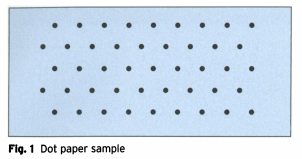
\includegraphics[width=0.33\textwidth]{sierp_fig_1}
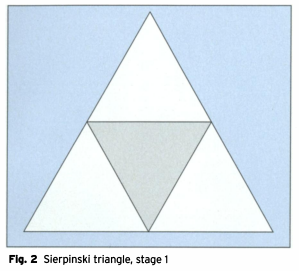
\includegraphics[width=0.33\textwidth]{sierp_fig_2}
\end{center}
To keep overzealous students from merely connecting every dot on the page, students should shade in this newly formed triangle. Next, students connect all the midpoints of the unshaded triangles, forming 3 new triangles, which they should shade in (see fig. 3).
\begin{center}
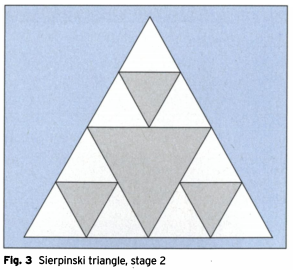
\includegraphics[width=0.33\textwidth]{sierp_fig_3}
\end{center}
This process can be continued indefinitely (although the students lose the benefit of the dots after stage 4, since the starting triangle has sides of length 16), as shown in the following figures:
\begin{center}
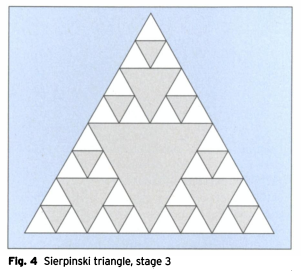
\includegraphics[width=0.33\textwidth]{sierp_fig_4}
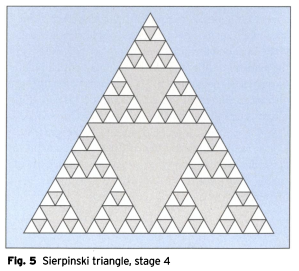
\includegraphics[width=0.33\textwidth]{sierp_fig_5}
\end{center}
%should the illustrations be cited in-line?
Students completing this activity are often surprised at how quickly the number of triangles grows. The growth is exponential, giving the student $3^{(n-1)}$ more triangles to shade at each step. 

In an introductory course to ordinary differential equations, a student is introduced to some very simple models which can be useful in science, the most elementary model being 
$$\frac{dx}{dt}=kx,$$
whose solution is precisely what we've been discussing, 
$$x(t)=e^{kt}$$
which is exponential growth. 

In actual practice however, models often require quite a bit of "ugliness" to be actually useful. A differential equation may have many parameters, or it may have nonlinear terms such as $\sin$, $\sqrt{\phantom{x}}$, or other parts that make the system difficult to deal with. 

In this paper, the reader will find an introduction to some
graphical and intuitive methods for dealing with nonlinear differential equations. This takes much of the "ugliness" and tackles it with pictures, making the problem much more digestible. We will see how these methods can be applied to biology, exploring a population model that uses a nonlinear term to represent the effect of fear on the population of the prey. 

\section{Using Differential Equations}

%A. What is a differential equation? How do you solve one, and what do its solutions mean? Very brief mention of the usual methods of solving them, emphasising that the advantage of the methods of this paper is that they avoid the textbook methods.

While in-depth study of this topic would likely necessitate taking a full course on differential equations, we get our feet wet with a basic introduction and a few definitions. A \emph{differential equation} describes a real life system by, instead of giving an equation which represents its location or state, giving an equation for how its state is changing. For example, in the equation 
\begin{equation}
\frac{dx}{dt}=x,
\end{equation}
the change in $x$ as time $t$ changes is equal to the actual value of $x$. That is, as $x$ grows, the rate of growth of $x$ also grows. A \emph{solution} to a differential equation is an explicit function which gives $x$ as a function of $t$, and which satisfies the differential equation. A solution to (1) is shown below, with $x$ on the vertical axis and $t$ on the horizontal axis:
\jpg{width=0.3\textwidth}{exp-x}
Look familiar? This is exponential growth, because the differential equation above can be solved as follows:
\[\begin{array}{rrcll}
&\dfrac{dx}{dt}&=&x\\
&\dfrac{1}{x}dx &=& dt & \text{separate the variables}\\
&\ln(x)&=&t+C& \text{integrate both sides}\\
\phantom{\text{exponentiate both sides}}&x&=&e^t e^C& \text{exponentiate both sides}\\
&x&=&x_0 e^t& \text{explanation below}\\
\end{array}\]
It turns out that $e^C$ is the initial value of $x$, so we notate it $x_0$ (to see this, try plugging in $t=0$). This process above is fairly straightforward if you're comfortable with calculus, but can you imagine trying to solve something like 
$$\dfrac{dx}{dt}=x\left[r-a(x-b)^2\right]$$
using a similar method? \footnote{This is one formulation of the Alee effect. In this equation, $a,b,$ and $r$ are constants. See Strogatz section 2.3 for more.} Suffice it to say, symbolic methods are important, but not always an effective way to solve real-life differential equations. 

\section{A Geometric Way of Thinking}

%B. Introduction to Strogatz’s method of exploring the basic qualities of a nonlinear system by graphing, and aided by elementary calculus. 

In his book, \textit{Nonlinear Dynamics and Chaos}, Steven Strogatz gives a brilliantly intuitive way of dealing with with differential equations, using pictures. Consider the following example \citep{strogatz_1994}:
\begin{equation}
\dot{x}=\sin x.
\end{equation}
(By the way, we will simplify the notation from now on by writing $\dot{x}$ to mean $\frac{dx}{dt}$.) This equation is solvable using the symbolic strategy we used for (1), although many nonlinear systems are impossible to solve in closed-form. However, the solution would fit many people's definition of "ugly":
\begin{equation}
t=\ln\left|\frac{\csc x_0 + \cot x_0}{\csc x + \cot x}\right|.
\end{equation}
While correct, this result is in many ways unhelpful. For example, what does $x(t)$ do as $t\to\infty$? This is a basic question we might ask about any system, and it is difficult to say without a computer-generated plot.

Instead, let us take a graphical approach. The funtion $\sin x$ is very easy to graph, and graphing $\dot{x}$ versus $x$ reveals a lot of information about the system. If we think of $x$ as the position of an imaginary particle on the horizontal axis, then $\dot{x}$ tells us the velocity of that particle. 
\jpg{width=0.75\textwidth}{stro_fig_2-1-1}
On the figure here (Figure 2.1.1 in \cite{strogatz_1994}), the arrows show that when $\dot{x}$ is positive, $x$ is moving to the right; and when $\dot{x}$ is negative, $x$ is moving to the left. This allows us to very easily answer our question from earlier- what happens as $t\to\infty$? By following the arrows, you can see that given any starting point, $x$ will move away from a hollow point and towards a solid point. At those points, $\dot{x}=0$, which means that $x$ doesn't move. These points are called \emph{fixed points}. As you can see, there are two kinds of fixed points. The solid dots in the picture represent \emph{stable} fixed points, because any point nearby will "settle in" towards such a fixed point. The hollow dots are called \emph{unstable} fixed points, because while starting exactly on an unstable fixed point will result in no movement, even a tiny perturbation to one side or the other will cause the state of the system, or the \emph{phase}, to move away from the unstable fixed point. 

You may notice that the picture is sloping upward at all the unstable fixed points, and downward at the stable ones. This means that we can obtain quite a lot of information about a system using just a bit of calculus. If your system is 
$$\dot{x}=f(x),$$
then all the fixed points can be found by solving $f(x)=0$, and one can determine their stability using the derivative:
\[\text{A fixed point } x^* \text{ is} \quad
\begin{cases}
\text{stable} & \text{if } f'(x^*)<0\\
\text{unstable} & \text{if } f'(x^*)>0\\
\end{cases}
\]

\section{Getting a Model "Dialed-In"}

%C. Definition of stable and unstable fixed points, also definition and illustration of a bifurcation using graphs of a quadratic equation, as in Edwards’ paper (with help from Desmos, and section 3.1 in Strogatz). 

Now that we've covered the basics of analyzing these sorts of problems, let's talk about creating a differential equation to use as a biological model. In order for our model to accurately represent the real-life situation, we'll need to involve accurate numbers. To do this, we use parameters. A parameter is a number that is constant within a specific system, but may chance between different applications. For example, a thrown ball and a catapult projectile can both be modeled with parabolas, but the two will require dramatically different numbers. This concept applies to differential equations as well. As an illustration, let's consider the differential equation
\begin{equation}
\dot{x}=ax^2+bx+c.
\end{equation}

\cite{edwards_2009} outline a fantastic method to explore the question "What happens to the graph as we change $a, b$, and $c$?" Edwards suggests using technology to vary the three parameters using sliders, and although he uses an old TI computer algebra system, we will demonstrate his method using Desmos \citep{desmos}. 

\noindent First, we input the equation, and assign a slider to each parameter. 
\jpg{width=0.5\textwidth}{desmos_1}
The reader is probably already familiar with the effects of changing the $a$ and $c$ parameters, as they are often used in graphing parabolas by hand. Varying $a$ stretches the graph, and changing $c$ causes a vertical shift. Notice how the vertex follows the dotted line as $c$ is changed. 
\begin{center}
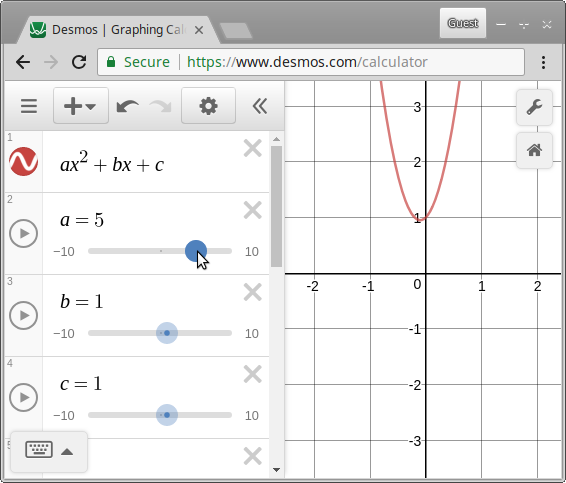
\includegraphics[width=0.45\textwidth]{desmos_2}
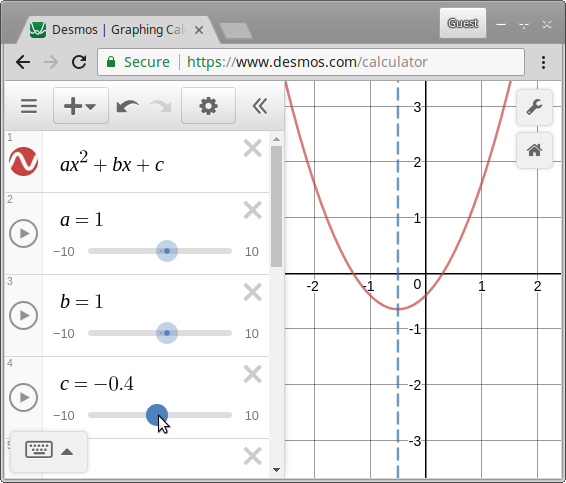
\includegraphics[width=0.45\textwidth]{desmos_3}
\end{center}
What happens when we vary $c$? If you try it, you'll see that the graph shifts around, but not in a linear way. You may not see it at first, but amazingly, the vertex actually traces out an inverted parabola! Try this at home, starting out with different $a$ and $c$ values, to see how the vertex always traces out a parabola as $b$ is varied. 
\begin{center}
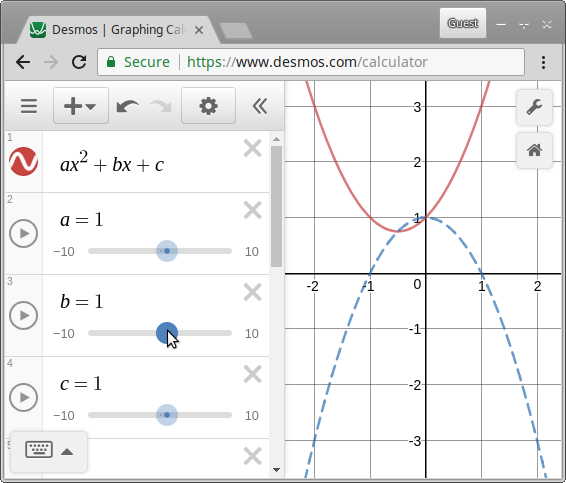
\includegraphics[width=0.3\textwidth]{desmos_4}
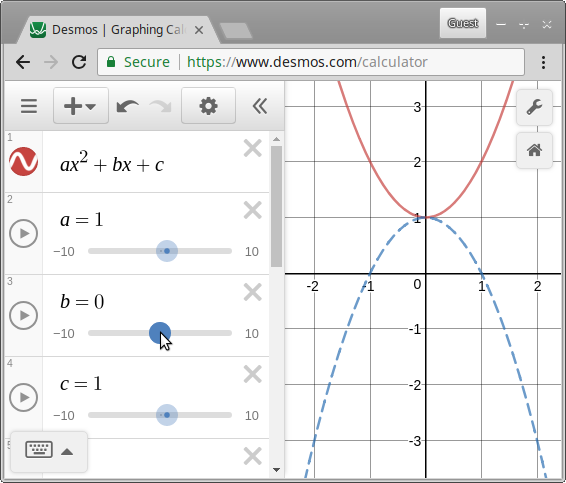
\includegraphics[width=0.3\textwidth]{desmos_5}
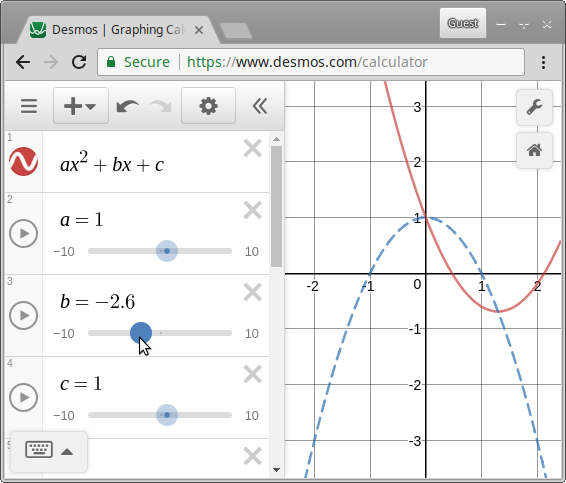
\includegraphics[width=0.3\textwidth]{desmos_6}
\end{center}
You may be asking yourself, "How does this relate to differential equations?" Well, when we interpret this parabola as a graph of $\dot{x}$ versus $x$, we'll see that something very interesting happens with the stable points when one or more of those parameters are changed. Consider this phase portrait of $\dot{x}=x^2-1$, from the \cite{strogatz_1994} text. 
\jpg{width=0.5\textwidth}{stro_fig_2-2-2}
You can see that it has two fixed points, one stable and one unstable. What if we thought of this as a specific case of $\dot{x}=r+x^2$, where $r=-1$? What happens when we vary the parameter $r$?
\jpg{width=0.95\textwidth}{stro_fig_3-1-1}
As you can see, when r is increased enough, the two fixed points merge into one, and then seem to annihilate each other. This is called a \emph{saddle-node bifurcation}, and it is a very important type of bifurcation. Imagine if, for example, a population had a stable fixed point, and a change in a parameter caused the fixed point to disappear? The population would either increase or decrease until it settled into another fixed point, which would have major biological implications. 

\section{The Logistic Model}

%D. Introduction to the Logistic Model, as per Brauer. This model can be much more easily analyzed via the graphical methods of Strogatz.

Now that we have all the tools we will need to apply this idea to science, let's explore an actual model. In this section, we will follow the exposition given in the textbook \textit{Mathematical models in population biology and epidemiology} \citep{brauer_2014}. To establish our notation, $x(t)$ denotes the size of the population at time $t$, and $\dot{x}$ the rate of change of the population with respect to time. At this point, we assume that the population growth rate depends on its size (more organisms will reproduce faster, as in the dice rolling example from earlier) and nothing else. This is a pretty reasonable assumption if we're talking about microorganisms like bacteria, but it would be too simple for anything more complicated like plants, animals, or people. To fully account for all of the different factors which may speed or slow population growth in more complex species, a model might need to account for competition within the species (overpopulation should reduce growth), or age structure (what if the death rate only depends on the number of old organisms, and young ones can be neglected?). It could also be the case that the population growth depends heavily on the population of another species as well as its own if there is competition or predation (or both) going on. 

Since the only variable we're only considering is $x$, our population, how can we model it? We've already thought in depth about the simplest type of model $\dot{x}=Cx$, where the growth rate is assumed to be a constant multiple of the population. In other words, the \emph{growth rate per capita} $\dot{x}(t)/{x}(t)$ is constant. Of course, if we're interested in modeling real-life populations, not even bacteria can grow exponentially for very long. There should be some point at which the population can't grow any more, either because there is no more room in the petri dish, or they have eaten all the food, or for some other reason. The simplest way to model this is to assume that the per capita growth rate starts out at some quantity $\lambda$, and then decreases as the population grows. This gives the famous \emph{logistic equation} 
\begin{equation}
\dot{x}=x(\lambda-ax).
\end{equation}
We can also rearrange this, to represent the maximum population. If $x$ is close to $0$, then the growth rate with be the largest, and then it will steadily decrease until the population reaches a certain amount. This alternate formulation is written 
\begin{equation}
\dot{x}=rx\left(1-\frac{x}{k}\right),
\end{equation}
Where $r=\lambda$ and $k=\lambda/a$. As you can see, when $x\approx0$, the second factor equals 1, and the population grows exponentially. But, as the population increases so that $x=k$, the second factor vanishes, and so does $\dot{x}$. $r$ is called the \emph{intrinsic growth rate}, and $k$ is called the \emph{carrying capacity}. The logistic equation is solvable symbolically (though it requires quite some effort). A few solutions are shown below \citep{brauer_2014}, to give the reader a visual idea of how the system behaves. 
\jpg{width=0.5\textwidth}{brauer_fig_1-1}
Could we have analyzed this system in some other way? Of course, let's use the graphical method of Strogatz. To get a better look, distribute the $x$ in equation (5). 
$$\dot{x} =-ax^2+\lambda x$$
Now we see that this is a parabola, with which we are well acquainted. In fact, we can even determine the location and stability of the fixed points in (5) without graphing. As we have previously mentioned, there is a fixed point $x^*$ wherever $\dot{x}=0$, so our fixed points lie at 
$x^*=0$
and 
$(\lambda-ax^*)=0$
or $x^*=\lambda/a$. To check the stability of these points, we only need determine if $f'(x^*)$ is positive or negative at each point. Since $f(x)=-ax^2+\lambda x$, $f'(x)=-2ax+\lambda$, then $f'(0)>0a$ as long as $\lambda>0$ (this has to be true, otherwise equation (5) doesn't make much sense), so $0$ is unstable. Also, $f'(\lambda/a)=-\lambda$, so this fixed point is stable for the same reason. 

The interpretation of all this is that, regardless of the specific values of the parameters $a$ and $\lambda$, we will always see a stable fixed point, representing the carrying capacity, and an unstable fixed point at $x=0$. 

\section{A (Slightly) More Complex Model}

%E. Slight modification of the logistic model, adding a predation/fear parameter, in the style of the paper by Wang (although here we use a simplified version).

As we mentioned earlier, the logistic model does a great job for modeling population growth of very simple organisms, but should be augmented to model more complex organisms. In their paper "Modelling the fear effect in predator-prey
interactions", the authors explore just such a model \citep{wang_2016}. They start with three different parts:
$$\dot{x}=rx-dx-ax^2,$$
Where $r$ is the species' birth rate, $d$ is its
natural death rate, and $ax$ gives the death rate due to intra-species competition (notice how this last term has an $x$ in it; $a$ is really the parameter here, but it should makes sense to think of $-ax$ getting more negative as the population increases). Wang et al proceed to consider the population $y$ of predators in their model, including a predation term $-py$, but we will omit it for simplicity.

In the field, recent experiments have shown that predators can affect the population of prey in ways other than directly preying on them. For example, the prey could respond to its fear of predators by changing its habitat usage, foraging behavior, and sleep patterns. %more could be added here if necessary
To account for this, Wang et al added a predation term $f(k,y)$ which gives the effect on birth rates as a function of fear level $k$ and predator population $y$. To simplify the analysis, we will consider $f$ to be a parameter, and observe how it changes the dynamics. Thus, our latest model is given by 
$$\dot{x}=rx-dx-ax^2-f.$$

\section{Analyzing the Model}

%F. Through our graphical methods, we see that a bifurcation can happen as the rate of predation changes. If the predation rate grows too large, the stable fixed point disappears, and the population rate is negative everywhere, leading to extinction.

We can can rearrange the model above to simplify things. It is essentially a quadratic equation of the form 
$$\dot{x}=-ax^2+(r-d)x-f.$$
As we increase $f$ to represent stronger effect of fear, we see the same sort of situation we've seen before; a bifurcation. Increasing the value of $f$ causes a vertical shift in the graph. Observe what happens to the fixed points:
\begin{center}
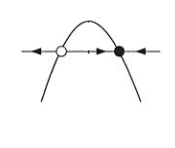
\includegraphics[width=0.3\textwidth]{stro_fig_3-1-1_rev_a}
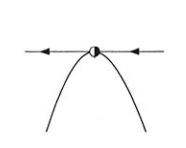
\includegraphics[width=0.3\textwidth]{stro_fig_3-1-1_rev_b}
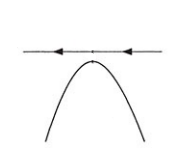
\includegraphics[width=0.3\textwidth]{stro_fig_3-1-1_rev_c}
\end{center}
As the effect of fear becomes stronger past a certain point (that is, when $f>\frac{r-d}{2a}$), the stable fixed point disappears and we see that the population decreases until the species becomes extinct.

\section{Conclusion} 
In this paper, we have seen a couple of classroom activities to explore exponential growth, which is the most basic population model. We also briefly discussed the definition and interpretation of a differential equation, and its usefulness in modeling populations. In our discussion of population models, we found that many functions which are useful modeling are not easy to analyze, but the graphical method of Strogatz gave us a very powerful and  very useful tool to use pictures to learn the qualitative aspects of the model, and an insight into bifurcations and how they work. Perhaps you can apply this graphical method to other biological questions as well.
% This is where the bibliography goes. Finish the body of your paper before this point, other than the appendix. 
\printbibliography
% I have commented out the appendix section since it isn't a standard for minimal documents. 
%\appendix 
\end{document}

  % ==============================================================
  %   Copyright (C) 2015  Jacob Long

  %   This program is free software: you can redistribute it and/or modify
  %   it under the terms of the GNU General Public License as published by
  %   the Free Software Foundation, either version 3 of the License, or
  %   (at your option) any later version.

  %   This program is distributed in the hope that it will be useful,
  %   but WITHOUT ANY WARRANTY; without even the implied warranty of
  %   MERCHANTABILITY or FITNESS FOR A PARTICULAR PURPOSE.  See the
  %   GNU General Public License for more details.

  %   You should have received a copy of the GNU General Public License
  %   along with this program.  If not, see <http://www.gnu.org/licenses/>.
  % ===============================================================
